\documentclass[a4paper,12pt]{article}
\usepackage[utf8]{inputenc}
\usepackage[german]{babel}
\usepackage[margin=2cm]{geometry}
\usepackage{url}
\usepackage{graphicx}
\usepackage{subcaption}
\usepackage{float}
\usepackage[bottom]{footmisc}

\title{Open Data Hub, Wetter-App}
\date{2020-02-18}
\author{Roland Bernard}

\begin{document}
\pagenumbering{arabic}
\maketitle
\newpage

\tableofcontents
\listoffigures
\newpage

Der Code für das Projekt und auch der \LaTeX-Quellcode dieses Berichts sind
auf dem Github-Repository unter \url{https://github.com/rolandbernard/suedtirol-weather}
zu finden.

\section{Idee und Zweck}
Ich habe mich dazu entschieden eine Wetter-App zu implementieren, welche die
Daten des Open Data Hub nutzt um Wetterinformationen bezüglich Südtirols
darzustellen. Die App bedient sich dabei der Daten der Mobilitäts API, um die
Momentanen Echtzeitdaten zu erhalten und der Tourismus API, um die Vorhersagen
zu bekommen. Das Ganze ist eine Webanwendung und als Single-Page-Applikation
implementiert. Die Anwendung hat drei größere Aufgaben. Einmal das Darstellen
einer Südtirolübersicht und Vorhersage (Abbildung \ref{fig:complete-overview}),
die Zweite Aufgabe ist das Anzeigen der momentanen Temperatur und der
Wettervorhersage für einen bestimmten Ort (Abbildung \ref{fig:complete-location})
und die letzte Funktionalität ist eine Karte auf der alle Stationen, deren
aktuelle und historische Messwerte übersichtlich dargestellt werden
(Abbildung \ref{fig:complete-stations}).

\begin{figure}[H]
    \centering
    \begin{subfigure}[b]{0.9\linewidth}
        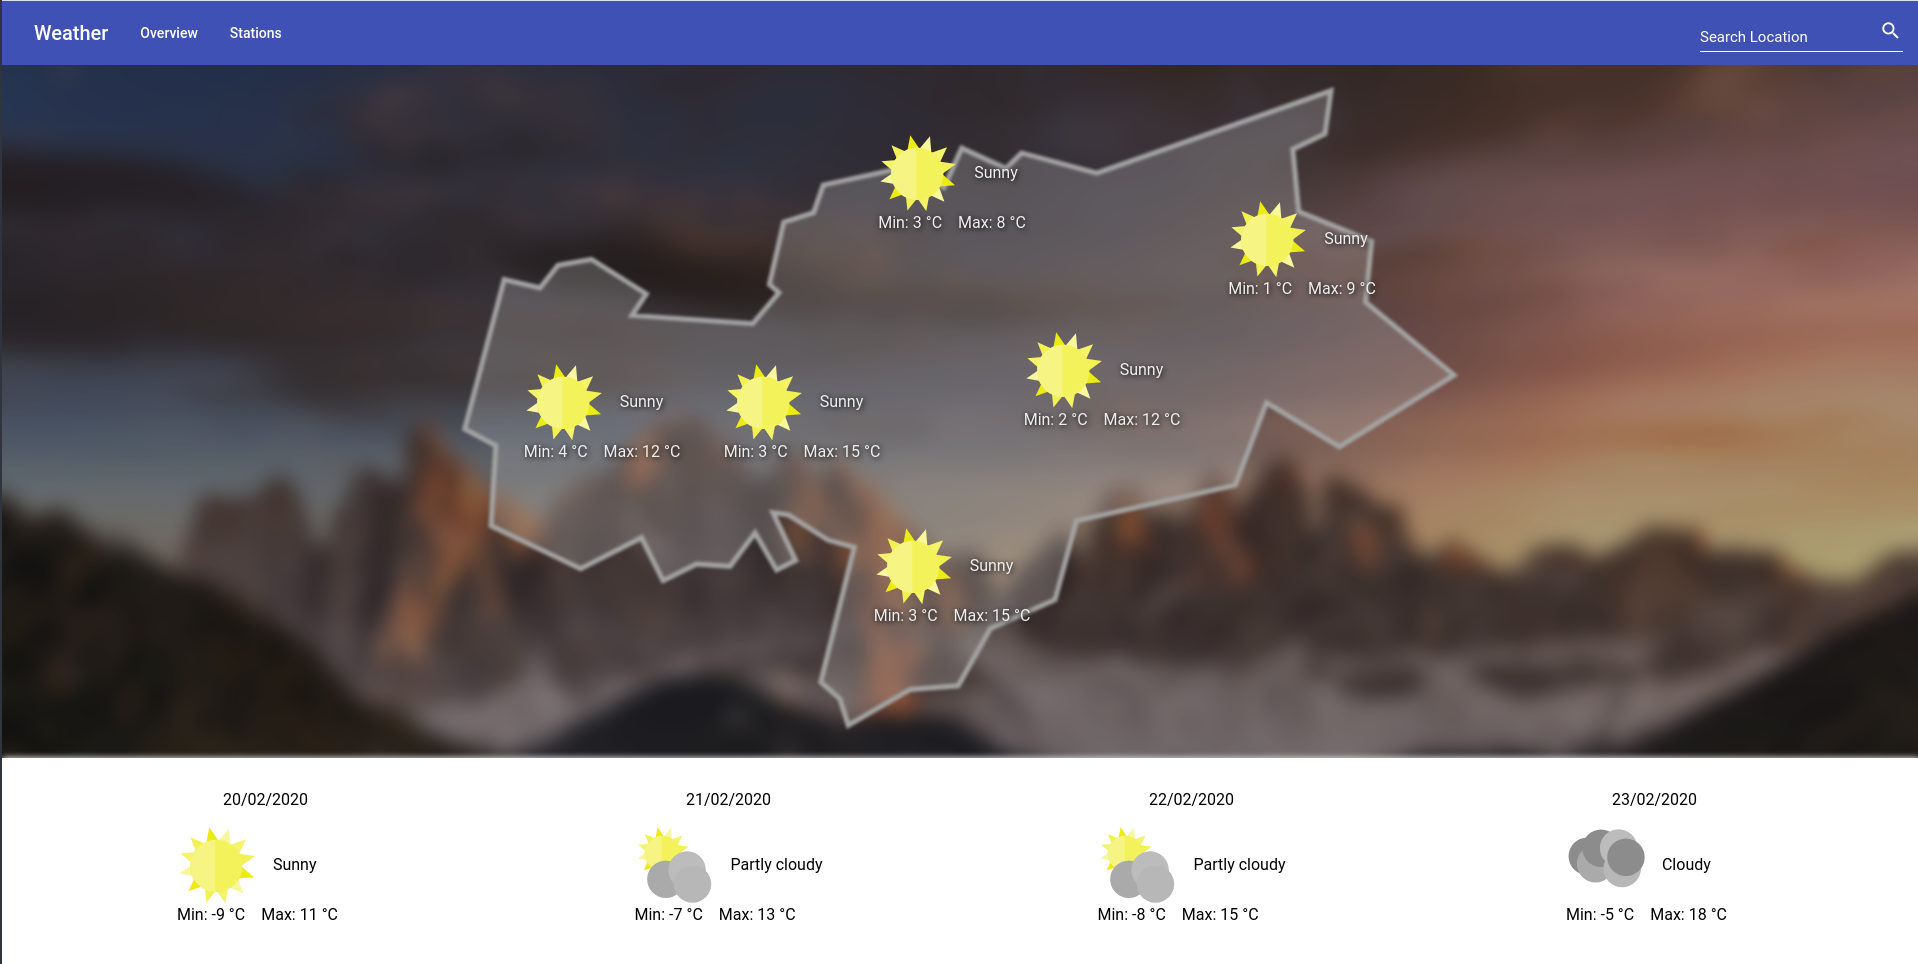
\includegraphics[width=\linewidth]{assets/complete-overview.png}
        \caption{Südtirolübersicht}
        \label{fig:complete-overview}
    \end{subfigure}
    \begin{subfigure}[b]{0.45\linewidth}
        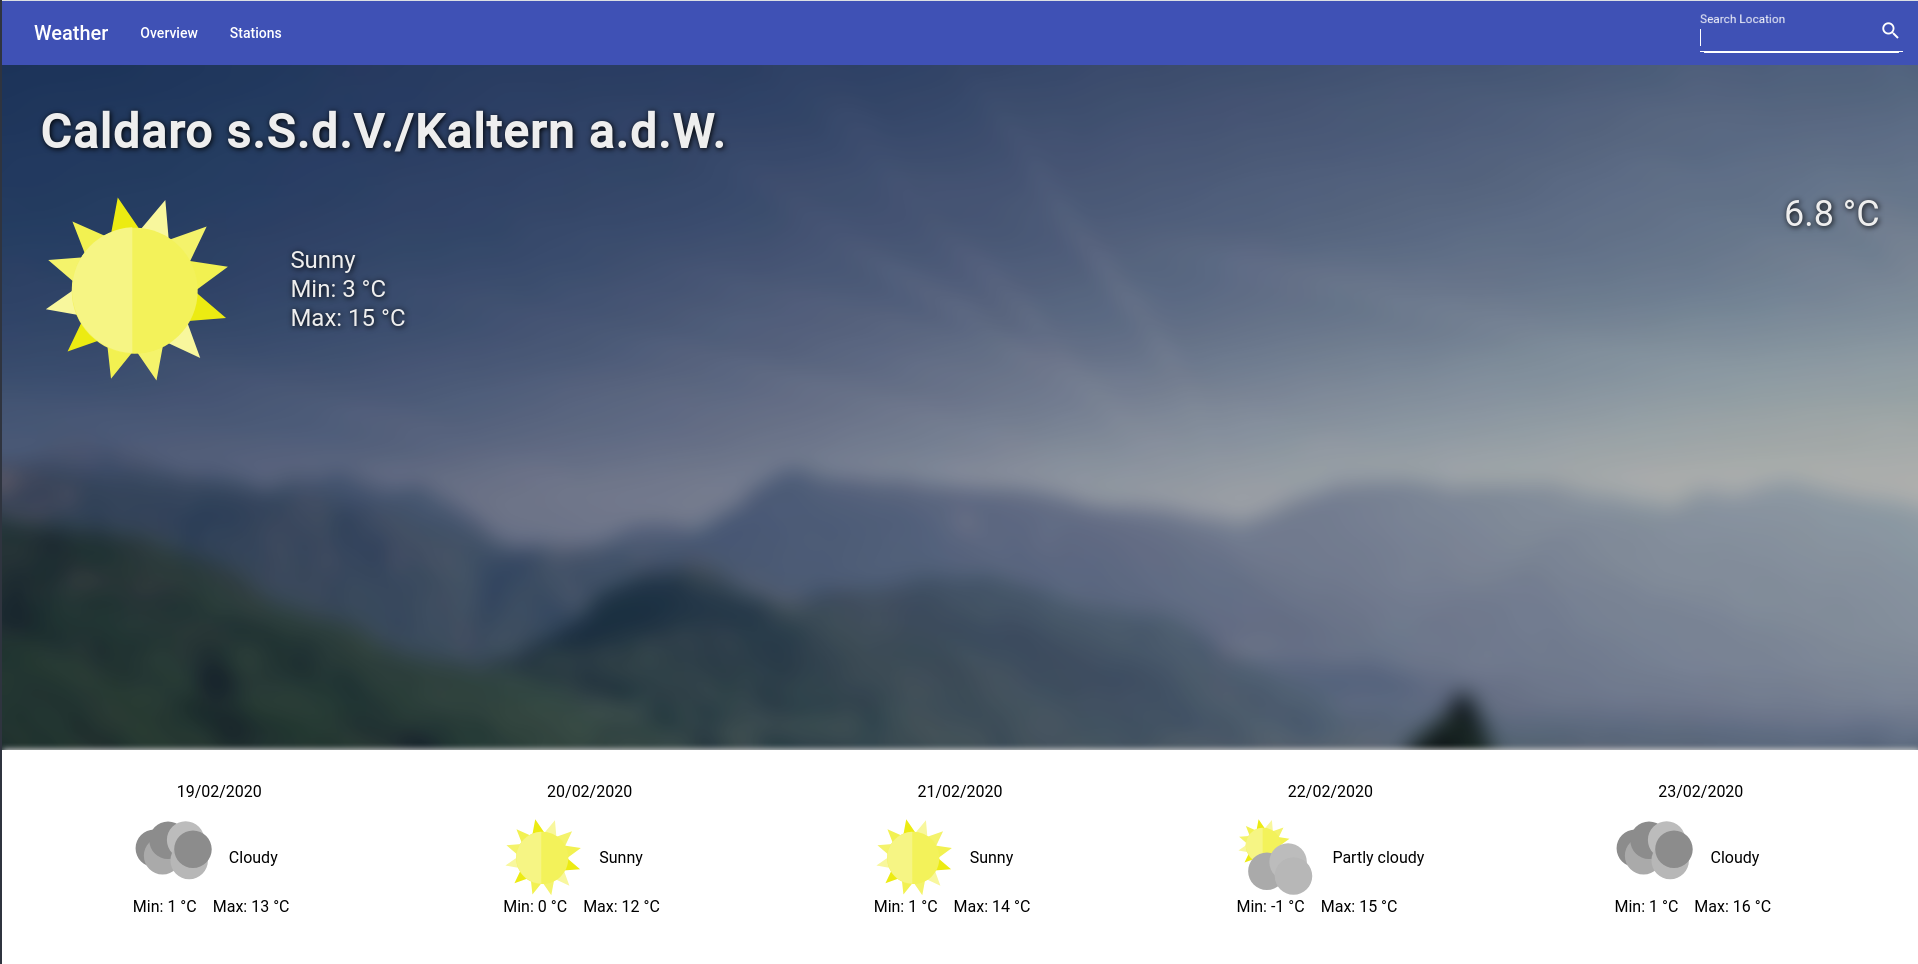
\includegraphics[width=\linewidth]{assets/complete-location.png}
        \caption{Wetter in einem bestimmten Ort}
        \label{fig:complete-location}
    \end{subfigure}
    \begin{subfigure}[b]{0.45\linewidth}
        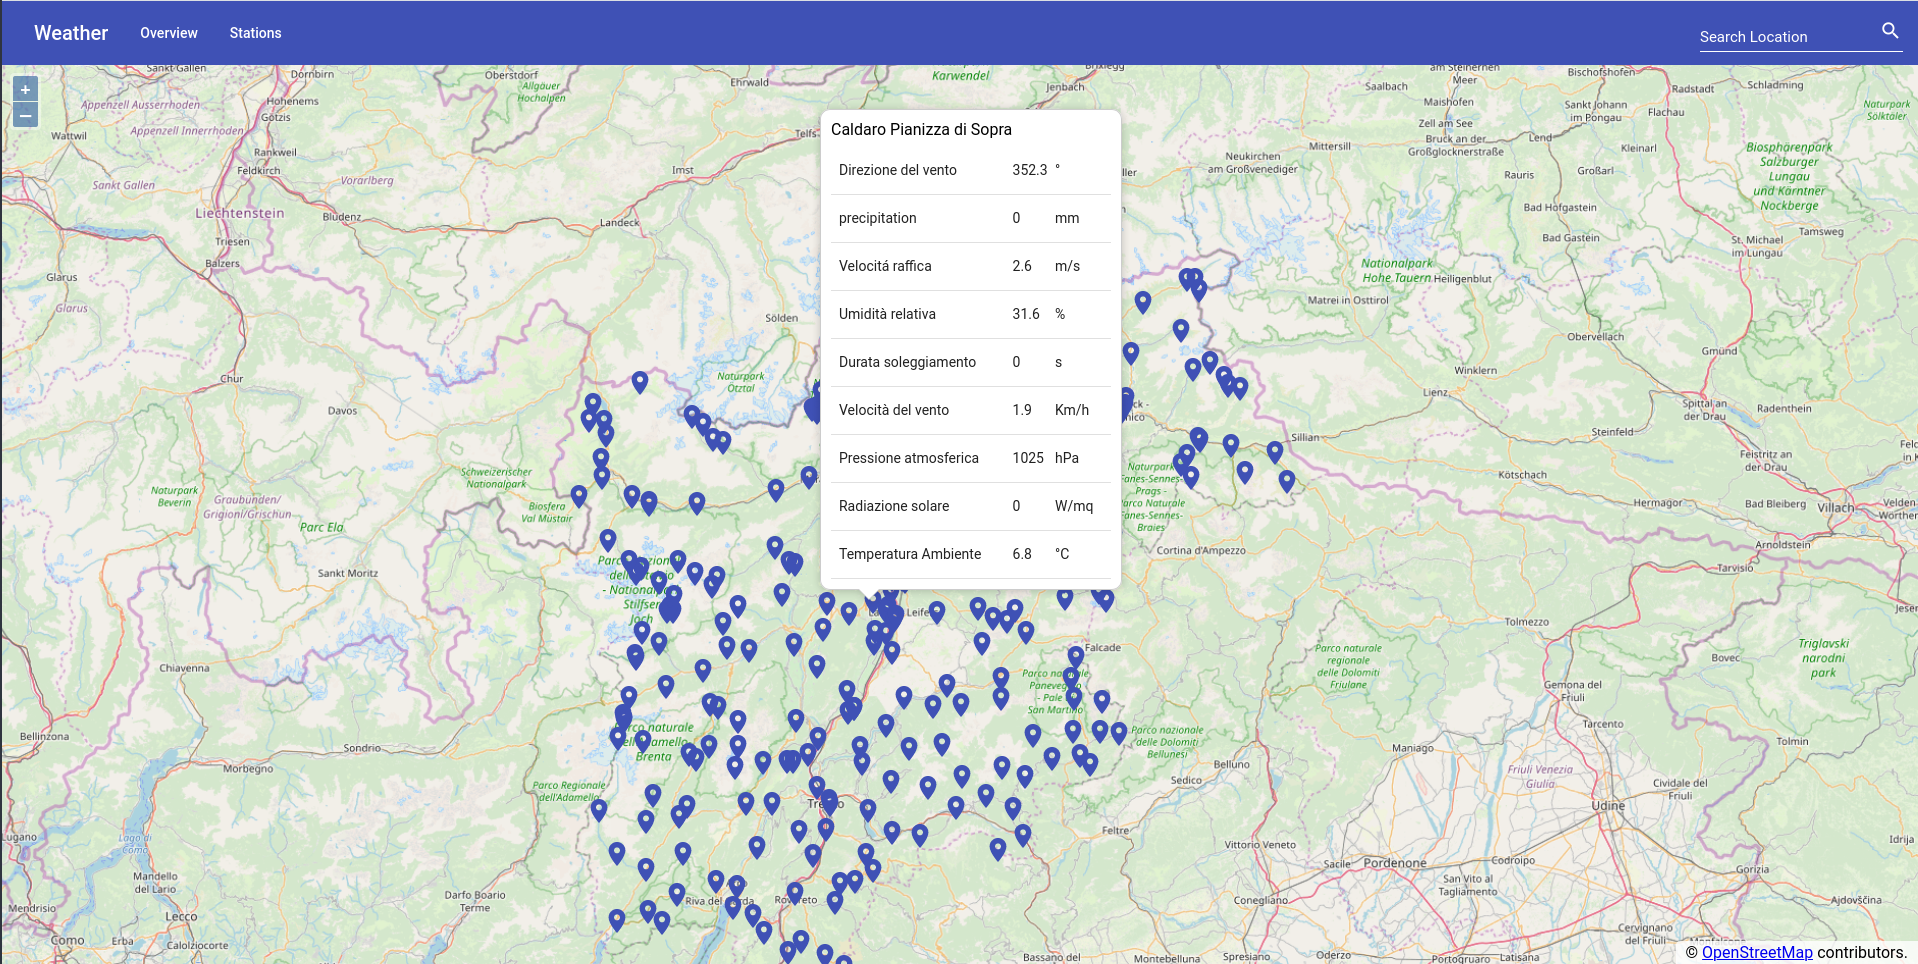
\includegraphics[width=\linewidth]{assets/complete-stations.png}
        \caption{Karte aller Stationen des ODH}
        \label{fig:complete-stations}
    \end{subfigure}
    \caption{Die einzelnen Funktionalitäten}
    \label{fig:complete}
\end{figure}

\section{Open Data Hub}
\begin{figure}[H]
    \centering
    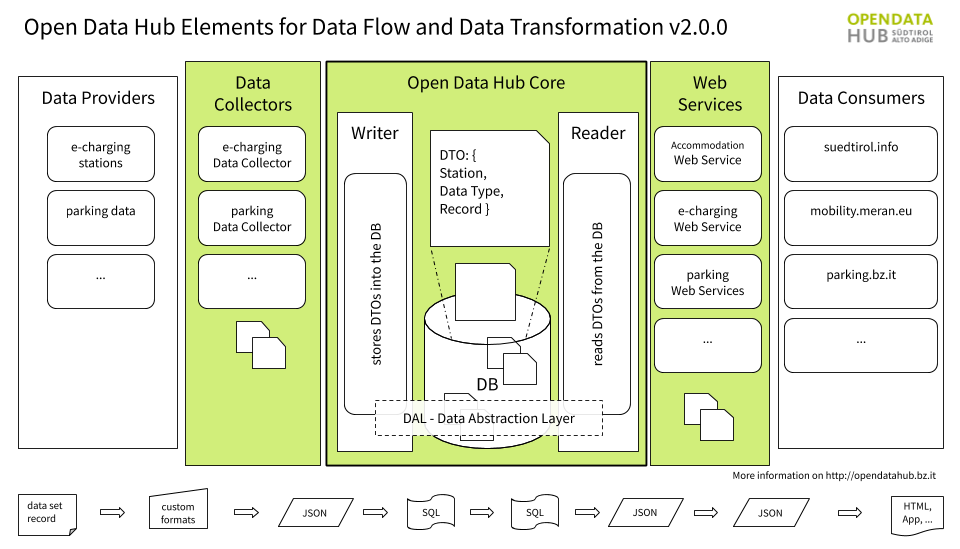
\includegraphics[width=\linewidth]{assets/odh-architecture.png}
    \caption{ODH Architekture \cite{web:odhdoc}}
    \label{fig:odharch}
\end{figure}

\subsection{Data Providers}
Die Data Providers sind außerhalb der Kontrolle des Open Data Hub Projekts.
Alle Daten, welche im Open Data Hub gespeichert werden, kommen ursprünglich
aus diesen Datenquellen. Die unterschiedlichen Data Providers können hierbei
unterschiedliche Formate und APIs benutzen. Die Data Provider können also zum
Beispiel eine REST-API zur Verfügung stellen oder aber auch nur über FTP
arbeiten.

\subsection{Data Collectors}
Im Open Data Hub sind die Data Collector dafür zuständig die Daten, welche die
Data Provider in verschiedenen Formaten zu Verfügung stellen, abzufragen und in
einem einheitlichen Format den DTO\footnote{\label{foo:dto}Data Transfer Object} an den Writer
weiterzugeben. Es gibt einen verschiedene Data Collector für verschiedene Data
Provider. Die Data Collectors sind im Git-Repository \texttt{bdp-commons}
\cite{web:bdpcommongit} definiert.

\subsection{Writer}
Die Writer sind dafür zuständig die Daten welche sie von den Data Collectors
erhalten mithilfe des DAL\footnote{\label{foo:dal}Data Abstraction Layer} in die Datenbank zu
schreiben. Implementiert sind die Writer im Git-Repository \texttt{bdp-core}
\cite{web:bdpcoregit}.

\subsection{Reader}
Die Aufgabe des Readers ist es die Daten mithilfe der DAL wieder aus der
Datenbank auszulesen und sie den Web-Services als DTO zu Verfügung zu stellen.
Wie auch die Writer sind sie in \texttt{bdp-core} \cite{web:bdpcoregit} definiert.

\subsection{Web Services}
Die Web Services stellen die Daten welche sie von dem Reader bekommen als
REST-API zur Verfügung. Die Data Consumer können diese Schnittstelle dann nutzen
um die Daten abzufragen.

\subsection{Data Consumers}
Data Consumers sind die Anwendungen, die die Daten des Open Data Hub
schlussendlich nutzen. Sie benutzen die APIs der Web Services, um auf die Daten
zuzugreifen. Auch diese Wetter-App ist ein solcher Data Consumer.

\section{Technologien}
\begin{figure}[H]
    \centering
    \begin{subfigure}[b]{0.3\linewidth}
        
\includegraphics[width=0.8\linewidth]{assets/angular.png}
        \caption{Angular}
    \end{subfigure}
    \begin{subfigure}[b]{0.3\linewidth}
        
\includegraphics[width=0.8\linewidth]{assets/openlayers.png}
        \caption{OpenLayers}
    \end{subfigure}
    \begin{subfigure}[b]{0.3\linewidth}
        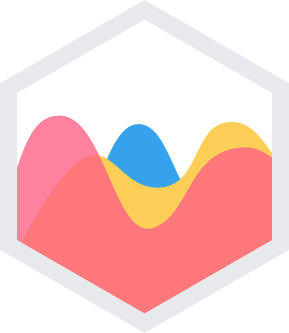
\includegraphics[width=0.8\linewidth]{assets/chartjs.png}
        \caption{Chart.js}
    \end{subfigure}
    \caption{Verwendete Technologien}
    \label{fig:technoligies}
\end{figure}

Die Webanwendung ist als Single-Page-Applikation mit dem Angular Framework
implementiert worden. Es wurden einige UI Elemente der Angular Material
Bibliothek verwendet. Um die Karte darzustellen wurde OpenLayers genutzt und um
die Diagramme darzustellen Chart.js.

\subsection{Angular}
Angular ist ein Komponentenbasiertes Framework zur Entwicklung von
Single-Page-Applikationen. Eine Anwendung besteht in Angular aus mehreren
Komponenten. Jede Komponente besteht aus einer TypeScript Datei einer HTML Datei
und einer Stylesheet Datei (in meinem Fall handelt es sich um SCSS Dateien). Ein
Angular Projekt muss zuerst kompiliert werden wobei nicht nur das TypeScript zu
JavaScript kompiliert werden muss, sondern auch die HTML und Stylesheet Dateien
kompiliert werden müssen.

\subsection{Angular Material}
Angular Material ist eine UI Bibliothek für Angular, welche mehrere vorgefertigte
Komponenten im Material Design zur Verfügung stellt. Durch das Verwenden einer
derartigen Bibliothek wird das Erstellen von Webanwendungen vereinfacht, weil
Standardkomponenten nicht selbst programmiert werden müssen. Auch gibt es den
Vorteil, dass das Aussehen bereits einheitlich nach dem Material Design gestaltet
ist.

\subsection{OpenLayers}
OpenLayers ist eine Bibliothek zum Anzeigen von Karten. OpenLayers hat eine
vielzahl an Features. Als Datenquelle für die Karte kann in OpenLayers recht
einfach auf die OpenStreetMap Karte zugegriffen werden. Damit OpenLayers gut mit
Angular verwendet werden kann, habe ich das \texttt{npm} Paket \texttt{ol} verwendet.

\subsection{Chart.js}
Chart.js ist eine Bibliothek welches es ermöglicht mithilfe von JavaScript
relativ einfach Diagramme zu erstellen.

\section{Architektur}
Die Aufgaben der Persistenzschicht werden in dieser Anwendung vollkommen vom
Open Data Hub übernommen. Selbst speichert die Anwendung nämlich keine Daten.
Die Anwendungsschicht ist hier relativ klein, weil nur wenig Logik benötigt wird,
um die Daten abzufragen und umzuwandeln. Diese Aufgaben werde von den Services
übernommen. Die Präsentationslogik wird dann schließlich von den Komponenten
implementiert.

\begin{figure}[H]
    \centering
    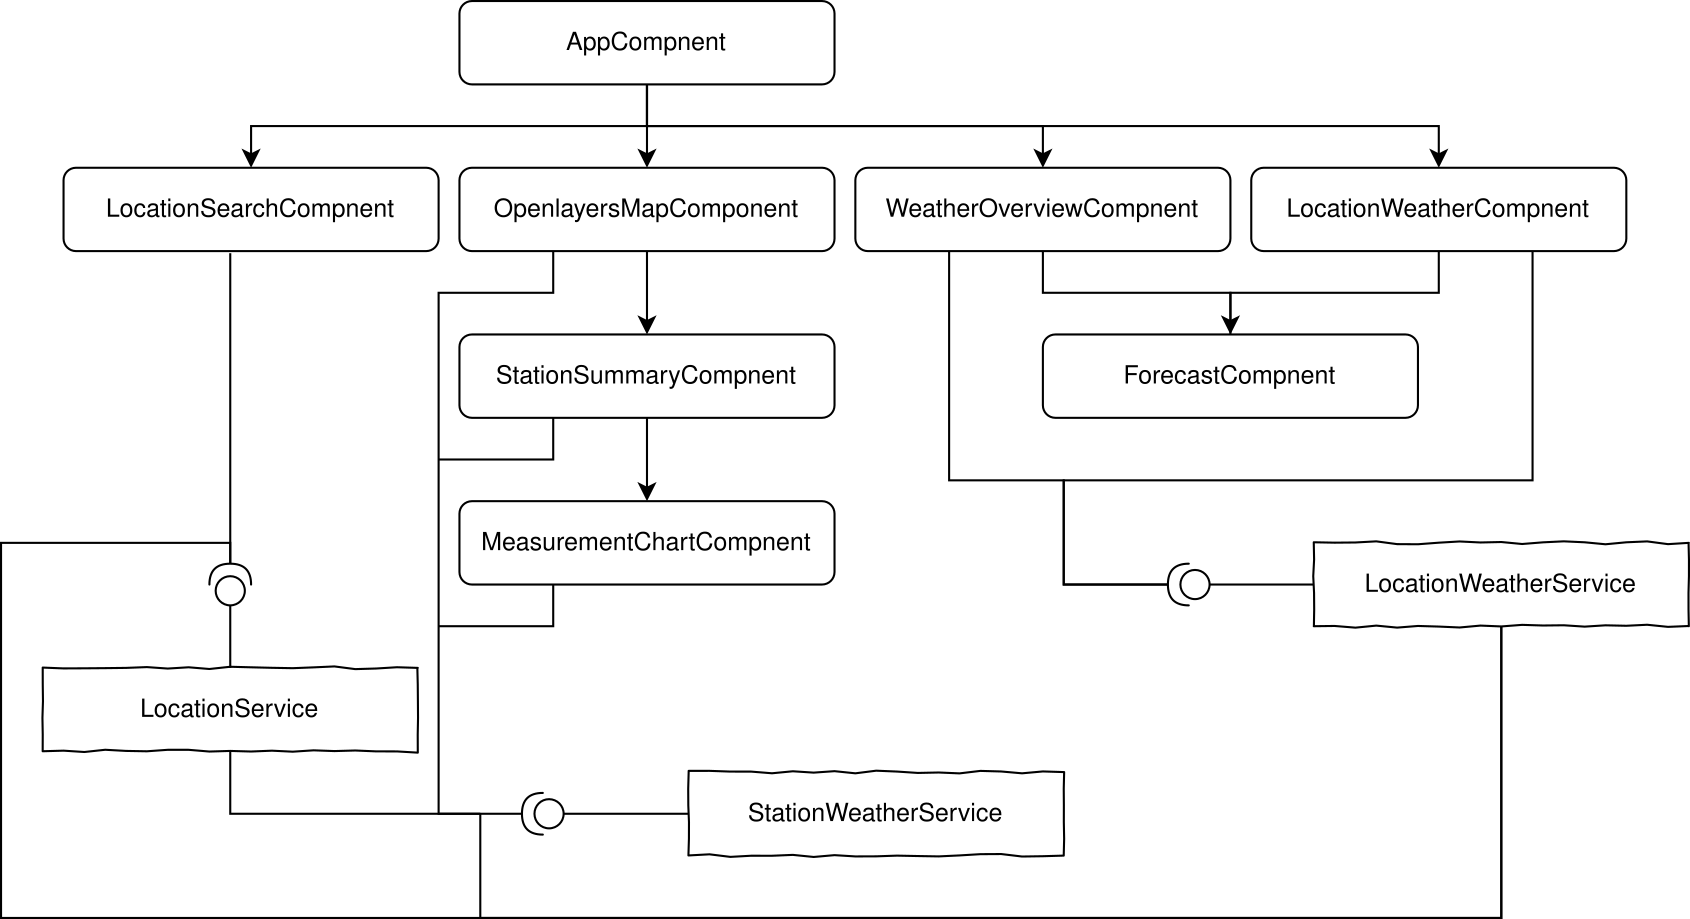
\includegraphics[width=\linewidth]{assets/wa-architecture.png}
    \caption{Architektur der Webanwendung}
    \label{fig:waarch}
\end{figure}

\subsection{Komponenten}
\subsubsection{AppComponent}
Die App-Komponente beinhaltet alle anderen Komponenten. Sie enthält die
Navigationsleiste und ein router-outlet, dessen Komponente sich ja nach
gewählter URI ändert.

\subsubsection{LocationSearchComponent}
\begin{figure}[H]
    \centering
    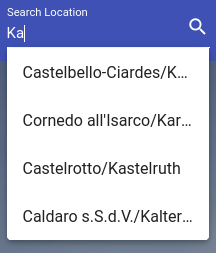
\includegraphics[width=0.2\linewidth]{assets/location-search.png}
    \caption{Ausgabe der LocationSearch-Komponente}
    \label{fig:location-search}
\end{figure}

Die LocationSearch-Komponente stellt ein Input-Feld zur verfügung, über welches
man nach Orten Suchen kann. Während man den Ortsnamen eingibt werden zusätzlich
Vervollständigungsvorschläge gegeben. Wählt der Nutzer einen der Vorschläge aus,
wird ein Event geworfen.

\subsubsection{OpenlayersMapComponent}
\begin{figure}[H]
    \centering
    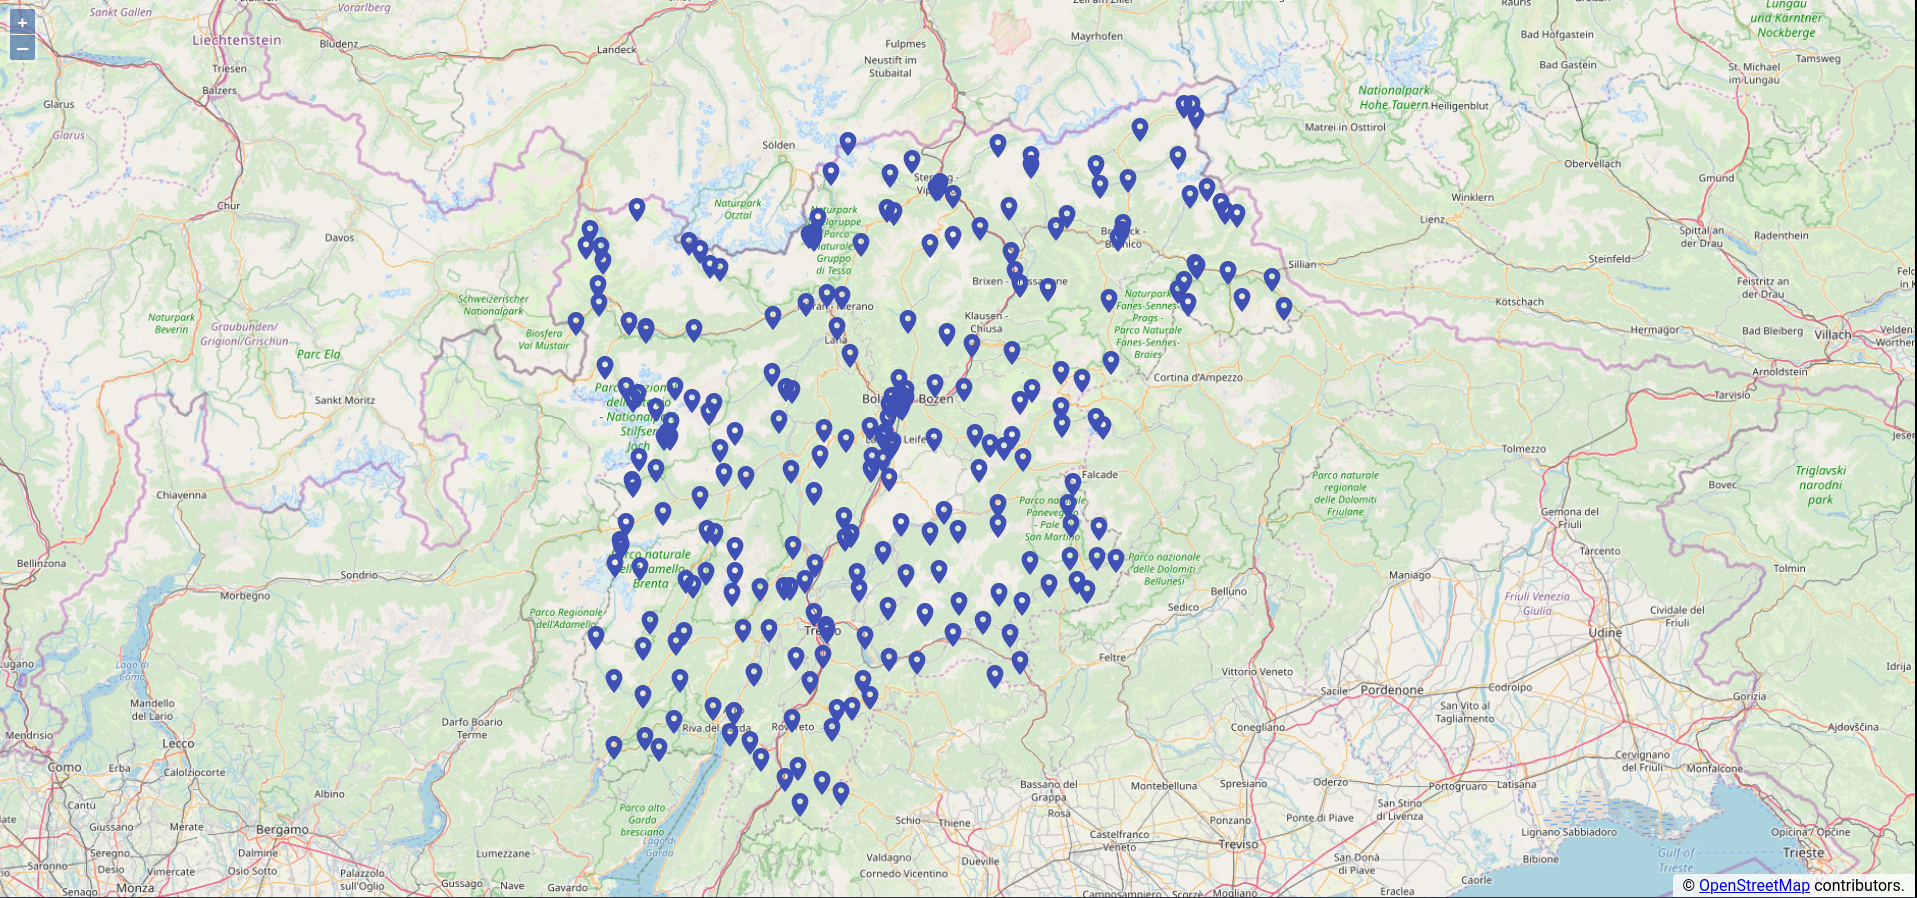
\includegraphics[width=0.9\linewidth]{assets/openlayers-map.png}
    \caption{Ausgabe der OpenlayersMap-Komponente}
    \label{fig:olenlayers-map}
\end{figure}

Die OpenlayersMap-Komponente zeigt eine Karte mithilfe von OpenLayers an, auf
welcher allen Stationen, welche vom Open Data Hub zur Verfügung gestellt werden,
angezeigt werven. Klickt man auf die Markierung einer Station wird ein Pop-up
geöffnet, welches die StationSummary-Komponente der jeweiligen Station enthält.
Zusätzlich ist es nicht möglich die Sicht der Karte von der Region um Südtirol
abzuwenden.

\subsubsection{StationSummaryComponent}
\begin{figure}[H]
    \centering
    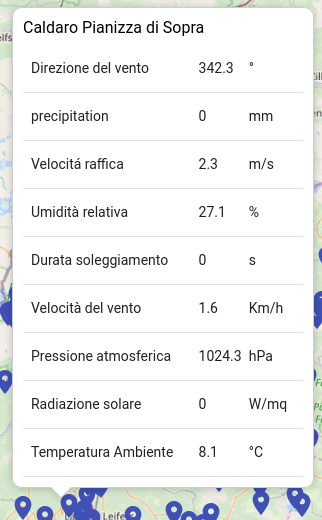
\includegraphics[width=0.3\linewidth]{assets/station-summary.png}
    \caption{Ausgabe der StationSummary-Komponente}
    \label{fig:station-summary}
\end{figure}

Die StationSummary-Komponente zeigt den Namen der darzustellenden Station und
alle momentanen Messwerte an. Wenn auf einen Messwert geklickt wird, wird eine
MeasurementChart-Komponente für den entsprechenden Messwert angezeigt.

\subsubsection{MeasurementChartComponent}
\begin{figure}[H]
    \centering
    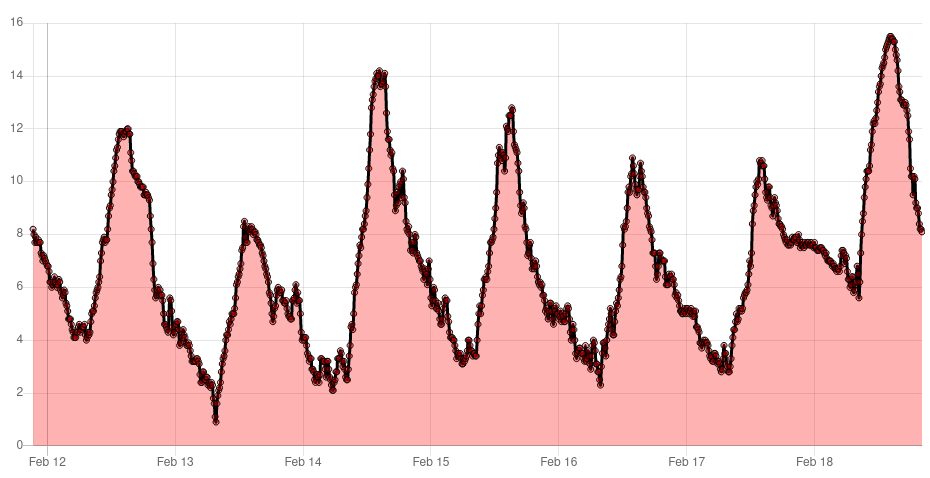
\includegraphics[width=0.8\linewidth]{assets/measurement-chart.png}
    \caption{Ausgabe der MeasurementChart-Komponente}
    \label{fig:measurement-chart}
\end{figure}

Die MeasurementChart-Komponente zeigt den Verlauf eines Messwerts einer bestimmten
Station über die letzten sieben Tage an. Zur Darstellung verwendet die Komponente
dabei Chart.js.

\subsubsection{WeatherOverviewComponent}
\begin{figure}[H]
    \centering
    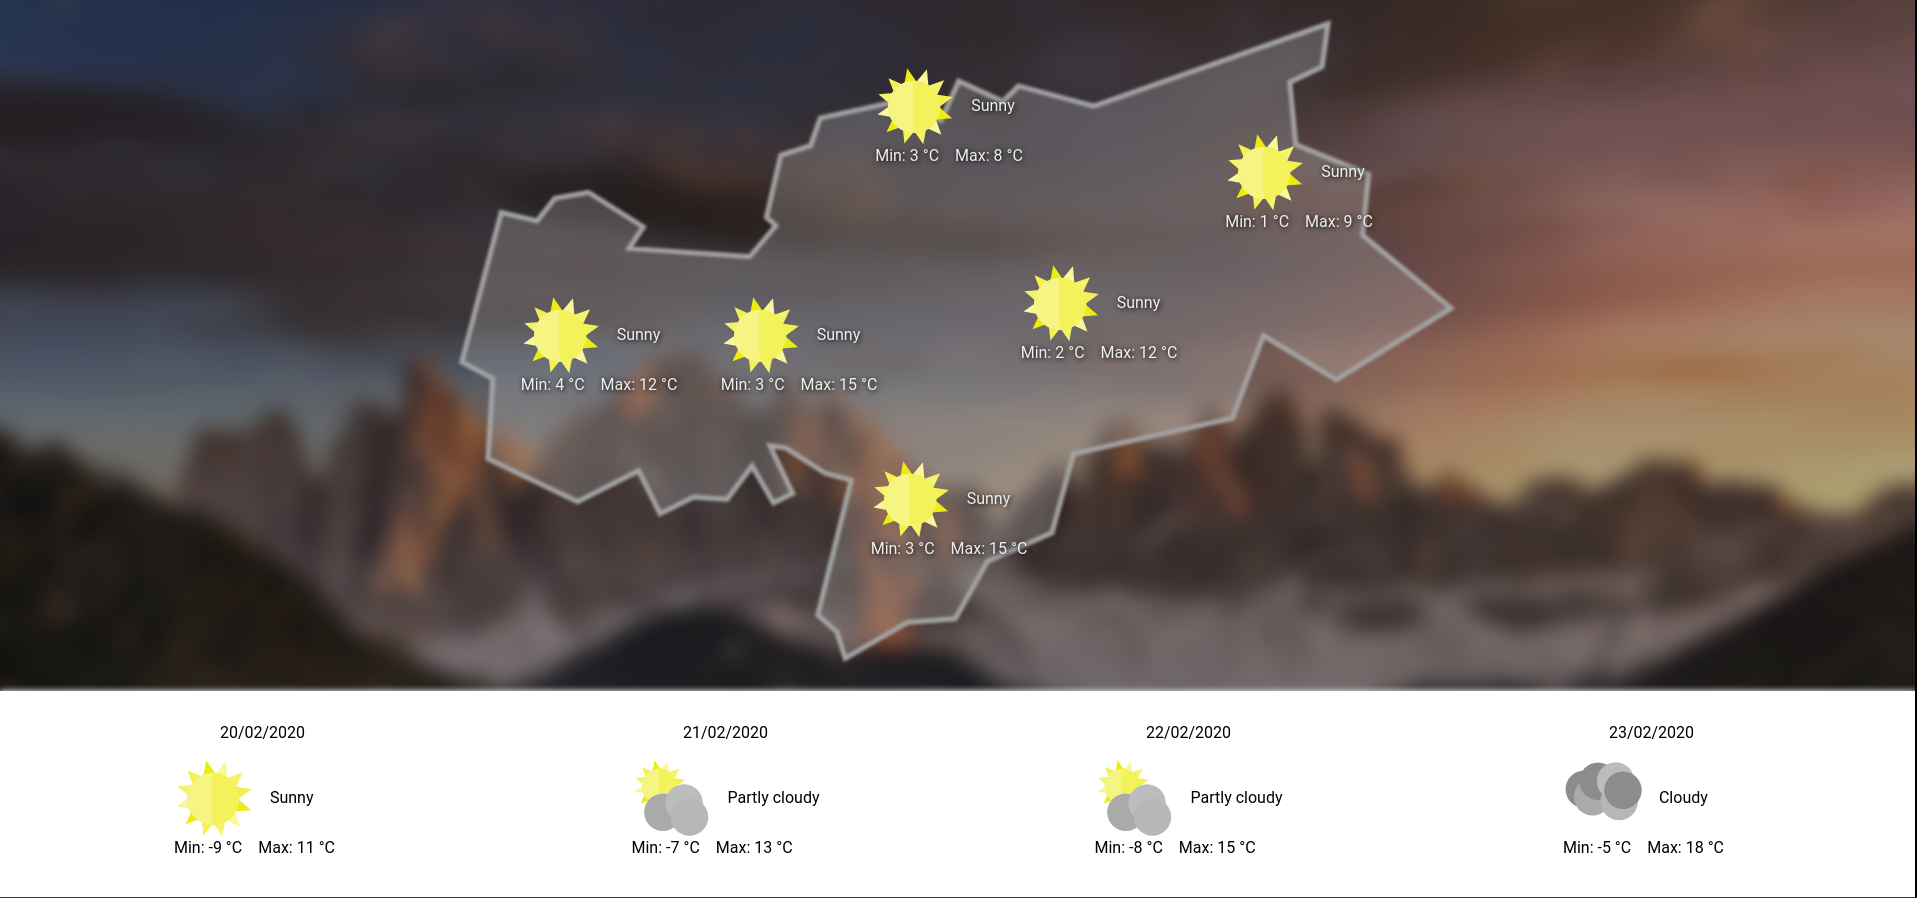
\includegraphics[width=0.9\linewidth]{assets/weather-overview.png}
    \caption{Ausgabe der WeatherOverview-Komponente}
    \label{fig:weather-overview}
\end{figure}

Die WeartherOverview-Komponente zeigt eine Südtirolübersicht der Wettervorhersage
an. Der heutige Tag wird dabei auf der Karte dargestellt und die folgenden vier
Tage werden darunter mithilfe der Forecast-Komponente dargestellt.

\subsubsection{LocationWeatherComponent}
\begin{figure}[H]
    \centering
    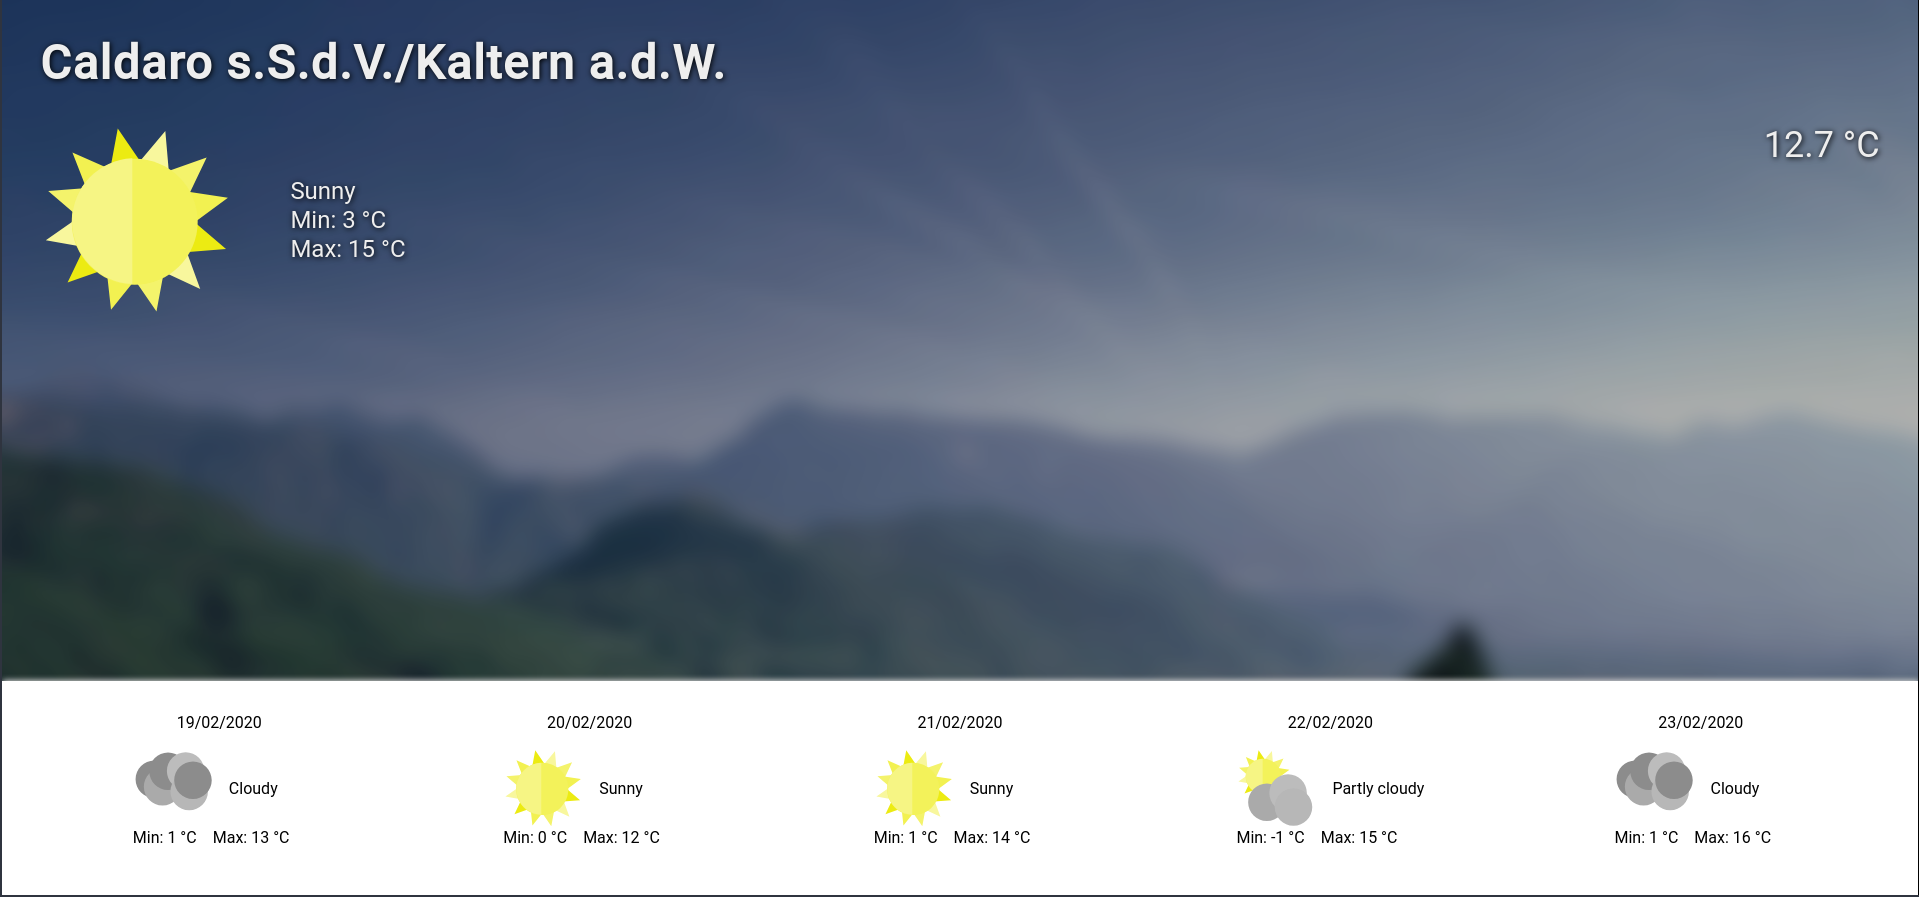
\includegraphics[width=0.9\linewidth]{assets/local-weather.png}
    \caption{Ausgabe der LocationWeather-Komponente}
    \label{fig:location-weater}
\end{figure}

Die LocationWeather-Komponente zeigt die Wettervorhersage und die aktuelle
Temperatur für einen bestimmten Ort an. Auch hier wird mithilfe der Forecast-Komponente
die Vorhersage für die kommenden Tage visualisiert. Der Hintergrund wird hier
je nach Ort anders gewählt.

\subsubsection{ForecastComponent}
\begin{figure}[H]
    \centering
    \begin{subfigure}[b]{0.4\linewidth}
        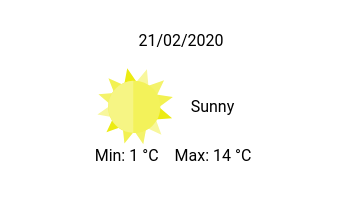
\includegraphics[width=\linewidth]{assets/forecast1.png}
        \caption{Sonnig}
    \end{subfigure}
    \begin{subfigure}[b]{0.4\linewidth}
        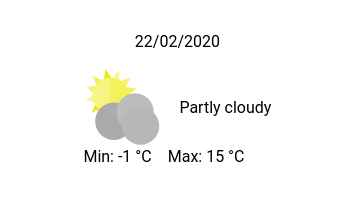
\includegraphics[width=\linewidth]{assets/forecast2.png}
        \caption{Teilweise bewölkt}
    \end{subfigure}
    \caption{Ausgabe der Forecast-Komponente}
    \label{fig:forecast}
\end{figure}

Die Forecast-Komponente dient zum Anzeigen eines Forecast-Objekts, welches
Informationen zum vorhergesagten Wetter eines Tages beinhaltet. Das
Forecast-Objekt wird der Komponente über das Attribut \texttt{forecast}
übergeben. Angezeigt wird die minimale und maximale Temperatur die erwartet
wird, die Wetterbeschreibung und ein Icon, welches zu dieser Beschreibung passt.

\subsection{Services}
\subsubsection{StationWeatherService}
Der StationWeather-Service nutzt die Daten der Mobilitäts API des Open Data Hubs.
Er besitzt Funktionen, um alle verfügbaren Stationen abzurufen, die von einer
Station zur Verfügung gestellte Messwerte zu bekommen und um die Werte eines
bestimmten Messwertes einer Station in der letzten Zeit zu ermitteln.

\subsubsection{LocationService}
Der Location-Service nutzt die Daten der Tourismus API des Open Data Hubs. Der
Service hat Funktionen, um die Orte in Südtirol zu ermitteln und auch eine Funktion
um von einem Ort auf die dazugehörige Wetter-Station zu gelangen. Diese Station
muss dann aber mit dem StationWeather-Service verwendet werden.

\subsubsection{LocationWeatherService}
Der LocationWeather-Service nutzt die Daten der Tourismus API des Open Data Hubs.
Er liefert die Wettervorhersagen sowohl für die Übersicht, als auch für die
einzelnen Orte. Wenn das Wetter für einen bestimmten Ort benötigt wird, wird
zusätzlich auch der StationWeather-Service abgefragt, um die aktuelle Temperatur
zu erfahren.

\newpage
\nocite{*}
\bibliography{report}
\bibliographystyle{ieeetr}
\end{document}
